\section{Example of symmetry affecting evaluation of electron paths}
In the main text we described the challenges of how to evaluate our model, as different electron paths can form the same products, for instance due to symmetry.
Figure \ref{fig:symmetric-reaction-example} is an example of this.


\begin{figure*}[h]

    \centering
    \begin{subfigure}[b]{0.95\textwidth}
        \centering
        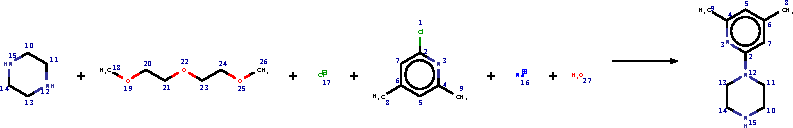
\includegraphics[width=\textwidth]{imgs/symmetry/main_reaction}
        \caption{Reaction as defined by USPTO SMILES}
    \end{subfigure}
    
    \par\bigskip % force a bit of vertical whitespace 
    \begin{subfigure}[b]{0.95\textwidth}
        \centering
        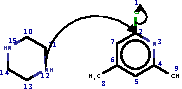
\includegraphics[width=0.4\textwidth]{imgs/symmetry/possible1}
        \qquad
        \qquad
        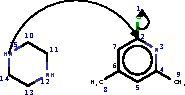
\includegraphics[width=0.4\textwidth]{imgs/symmetry/possible2}
        \caption{Possible action sequences that all result in same major product.}
    \end{subfigure}
    \caption{This example shows how symmetry can affect the evaluation of electron paths. In this example, although one electron path is given in the USPTO dataset, the initial N that reacts could be either 15 or 12, with no difference in the final product. This is why judging purely based on electron path accuracy can sometimes be misleading.}
    \label{fig:symmetric-reaction-example}
\end{figure*}

\section{Forming Node and Graph Embeddings}

In this section we briefly review existing work for forming node and graph embeddings, as well as describing more specific details relating to our particular implementation of these methods. Figure \ref{fig:graph_nn} provides a visualization of these techniques. 
We follow the main text by denoting a set of molecules as $\moleculeSet$, and refer to the atoms in these molecules (which are represented as nodes in a graph) as $\Ac$.


\begin{figure*}
\centering
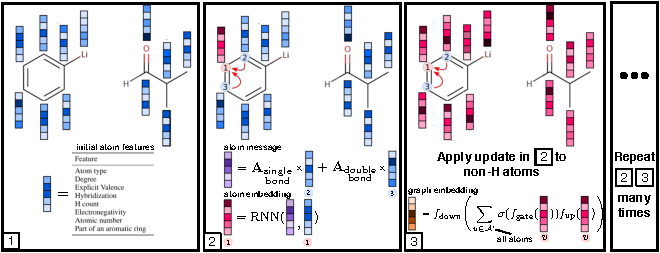
\includegraphics[width=\textwidth]{imgs/graph_nn}
\caption{
Visualization of how node embeddings and graph embeddings are formed. 
Node embeddings are $d$-dimensional vectors, one for each node. 
They are obtained using Gated Graph Neural Networks \citep{li2016gated}.
These networks consist of a series of iterative steps where the embeddings for each node are updated using the node's previous embedding and a message from its neighbors.
 Graph embeddings are $q$-dimensional vectors, representing a set of nodes, which could for instance be all the nodes in a particular graph \citep{li2018learning}.
  They are formed using a function on the weighted sum of node embeddings.
}
\label{fig:graph_nn}
\end{figure*}


 We start with Gated Graph Neural Networks (GGNNs) \citep{li2016gated, gilmer2017neural}, which we use for finding node embeddings.
 We denote these functions as $\fEmbed: \moleculeSet \to \mathbb{R}^{|\Ac|\times d}$, where we will refer to the output as the node embedding matrix, $\nodeEmbeddings{\moleculeSet} \in \mathbb{R}^{|\Ac|\times d}$. 
Each row of this node embedding matrix represents the embedding of a particular atom; the rows are ordered by atom-mapped number, a unique number assigned to each atom in a SMILES string.
The GGNN form these node embeddings through a recurrent operation on messages, $\mb_v$, with $v \in \Ac$, so that there is one message associated with each node.
At the first time step these messages, $\mb_v^{(0)}$, are initialized with the respective atom features shown in Table \ref{table:atom-features}. GGNNs then update these messages in a recursive nature:

\begin{align}
	\mb_v^{(s)} = \textrm{GRU}\left( 
					\mb_v^{(s - 1)},  
						\sum_{i \in \neigh{1}(v)} f_\textrm{single}\left(\mb_i^{(s - 1)}\right) +
						\sum_{j \in \neigh{2}(v)} f_\textrm{double}\left(\mb_j^{(s - 1)}\right) +
						\sum_{k \in \neigh{3}(v)} f_\textrm{triple}\left(\mb_k^{(s - 1)}\right)
					\right)
\end{align}

Where $\textrm{GRU}$ is a Gated Recurrent Unit \citep{Cho2014-xt}, the functions $\neigh{1}(v)$, $\neigh{2}(v)$, $\neigh{3}(v)$ index the nodes connected by single, double and triple bonds to node $v$ respectively and $f_\textrm{single}(\cdot)$, $f_\textrm{double}(\cdot)$ and $f_\textrm{triple}(\cdot)$ are linear transformations with learnable parameters.
This process continues for $S$ steps (where we choose $S=4$). In our implementation, messages and the hidden layer of the GRU have a dimensionality of 101, which is the same as the dimension of the raw atom features.
The node embeddings are set as the final message belonging to a node, so that indexing a row of the node embeddings matrix, $\nodeEmbeddings{\moleculeSet}$, gives a transpose of the final message vector, ie $[\nodeEmbeddings{\moleculeSet}]_v = \mb_v^{(S)t}$.

\begin{table}
  \caption{Atom features we use as input to the GGNN. These are calculated using RDKit.}
  \label{table:atom-features}
  \centering
  \begin{tabular}{ll}
    \toprule
    Feature     & Description      \\
    \midrule
    Atom type & 72 possible elements in total, one hot  \\
    Degree     & One hot (0,   1,   2,   3,   4,   5,   6,   7,  10)  \\
    Explicit Valence     & One hot   (0,   1,   2,   3,   4,   5,   6,   7,   8,  10,  12,  14)    \\
    Hybridization & One hot (SP, SP2, SP3, Other) \\
    H count & integer \\
    Electronegativity & float \\
    Atomic number & integer \\
    Part of an aromatic ring & boolean\\
    \bottomrule
  \end{tabular}
\end{table}


One can represent entire graphs with graph embeddings \citep{li2018learning,Johnson2017-pd}, which are $q$-dimensional vectors representing a set of nodes; i.e.\ an entire molecule or set of molecules.
These are computed by the function $\fEmbedGraphsInclFEmbed: \moleculeSet \to \mathbb{R}^{q}$. 
In practice the function we use consists of the composition of two functions: $\fEmbedGraphsInclFEmbed(\cdot) = (r \circ \fEmbed)(\cdot)$.

Having already introduced the function $\fEmbed(\cdot)$, we now introduce the function $r(\cdot)$.
This function, that maps a set of node features to  graph embeddings, $\fEmbedGraphs: \mathbb{R}^{|\Ac|\times d} \to \mathbb{R}^{q}$, is similar to the readout functions used for regressing on graphs detailed in \citep[Eq. 3]{gilmer2017neural} and the graph embeddings described in \citet[\S B.1]{li2018learning}. 
Specifically, $\fEmbedGraphs(\cdot)$ consists of three functions, $\fui(\cdot)$, $\fuj(\cdot)$ and $\fuk(\cdot)$, which could be any multi-layer perceptron (MLP) but in practice we find that linear functions suffice.
These three functions are used to form the graph embedding as so:
\begin{align}
	\fEmbedGraphs(\nodeEmbeddings{\moleculeSet_t}) = \fuk\left(\sum_{v \in \Ac'} \sigma\left(\fui([\nodeEmbeddings{\moleculeSet}]_v)\right) \fuj([\nodeEmbeddings{\moleculeSet}]_v)\right).
	\label{eq:graph-embedding}
\end{align}
Where $\sigma(\cdot)$ is a sigmoid function.
We can break this equation down into two stages.
In stage (i), similar to \citet[\S B.1]{li2018learning}, we form an embedding of one or more molecules (with vertices $\Ac'$ and with $\Ac' \subseteq  \Ac$) by performing a gated sum over the node features. 
In this manner the function $\fui(\cdot)$ is used to decide how much that node should contribute towards the embedding,
 and $\fuj(\cdot)$ projects the node embedding up to a higher dimensional space; following \citet[\S B.1]{li2018learning}, we choose this to be double the dimension of the node features.
Having formed this embedding of the graphs, we project this down to a lower $q$-dimensional space in stage (ii), which is done by the function $\fuk(\cdot)$. 







\section{More training details}

In this section we go through more specific model architecture and training details omitted from the main text. 

\subsection{Model architectures}
In this section we provide further details of our model architectures.

Section 3 of the main paper discusses our model.
In particular we are interested in computing three conditional probability terms: (1) $p_\theta^{\mathrm{start}}(a_0 \mid \moleculeSet_0, \moleculeSet_e)$, the probability of the initial state $a_0$ given the reactants and reagents; 
(2) the conditional probability $p_\theta(a_t \mid \moleculeSet_t, a_{t-1}, t)$  
of the next state $a_t$ given the intermediate products $\moleculeSet_t$ for $t > 0$;
and (3) the probability $p_\theta^{\mathrm{cont}}(c_{t} \mid \moleculeSet_{t})$ that the reaction continues at step $t$.

Each of these is parametrized by NNs. We can split up the components of these NNs into a series of modules: $\fCont(\cdot)$, $\fReag(\cdot)$, $\fAdd(\cdot)$, $\fRemove(\cdot)$ and $\fInitial(\cdot)$. 
All of these operate on node embeddings created by the same GGNN.
 In this section we shall go through each of these modules in turn.




As mentioned above (Eq. \ref{eq:graph-embedding}) both $\fCont(\cdot)$ and $\fReag(\cdot)$ (which following the explanation in the previous section, make up part of $\fContInclEm(\cdot)$ and $\fReagInclEm(\cdot)$ respectively) consist of three
linear functions. 
For  both, the function $\fui(\cdot)$ is used to decide how much each node should contribute towards the embedding and so projects down to a scalar value.
Again for both, $\fuj(\cdot)$ projects the node embedding up to a higher dimensional space, which we choose to be 202 dimensions. 
This is double the dimension of the node features, and similar to the approach taken by \citet[\S B.1]{li2018learning}.
Finally, $\fuk(\cdot)$ differs between the two modules, as for $\fCont(\cdot)$ it projects down to one dimension (ie $q=1$) (to later go through a sigmoid function and compute a stop probability), whereas for  $\fReag(\cdot)$, $\fuk(\cdot)$ projects  to a dimensionality of 100 (ie $q=100$) to form the reagent embedding.


The modules for $\fAdd(\cdot)$ and $\fRemove(\cdot)$, that operate on each node to produce an action logit, are both NNs consisting of one hidden layer of 100 units. 
Concatenated onto the node features going into these networks are the node features belonging to the previous atom on the path.



The final function, $\fInitial(\cdot)$, is represented by an NN with hidden layers of 100 units. 
When conditioning on reagents (ie for
 \ourModelR
 )
  the reagent embeddings calculated by $\fReag(\cdot)$ are concatenated onto the node embeddings and we use two hidden layers for our NN. When ignoring reagents (ie for \ourModelIR) we use one hidden layer for this network. In total \ourModelR has approximately 250,000 parameters and \ourModelIR has approximately 190,000.

Although we found choosing the first entry in the electron path is often the most challenging decision, and greatly benefits from reagent information, we also considered a version of \ourModel where we fed in the reagent information at every step.
In other words, the modules for $\fAdd(\cdot)$ and $\fRemove(\cdot)$ also received  the reagent embeddings calculated by $\fReag(\cdot)$ concatenated onto their inputs.
On the mechanism prediction task (Table \ref{table:mech-predict}) this gets a slightly improved top-1 accuracy of 78.4\% (77.8\% before) but a similar top-5 accuracy of 94.6\% (94.7\% before).
 On the reaction product prediction task (Table \ref{table:prod-predict}) we get 87.5\%, 94.4\% and 96.0\% top-1, 3 and 5 accuracies (87.0\%, 94.5\% and 95.9\% before). 
 The tradeoff is this model is somewhat more complicated and requires a greater number of parameters.

\subsection{Training}

We train everything using Adam \citep{kingma2014adam} and an initial learning rate of 0.0001, which we decay after 5 and 9 epochs by a factor of 0.1. 
We train for a total of 10 epochs.
For training we use reaction minibatch sizes of one, although these can consist of multiple intermediate graphs.






\section{Further details on identifying reactions with linear flow topology}
\label{sect:electron_path_identify}

This section provides further details on how we extract reactions with linear electron flow topology, complementing Figure \ref{fig:dataset_steps} in the main text. 
We start from the USPTO SMILES reaction string and bond changes and from this wish to find the electron path.

The first step is to look at the bond changes present in a reaction. 
Each atom on the ends of the path will be involved in exactly one bond change;
the atoms in the middle will be involved in two. 
We can then line up bond change pairs so that neighboring pairs have one atom in common,
 with this ordering forming a path.
For instance, given the pairs "\texttt{11-13, 14-10, 10-13}" we form the unordered path "\texttt{14-10, 10-13, 13-11}".
If we are unable to form such a path, for instance due to two paths being present as a result of multiple reaction stages, then we discard the reaction.

For training our model we want to find the ordering of our path, so that we know in which direction the electrons flow.
To do this we examine the changes of the properties of the atoms at the two ends of our path. 
In particular, we look at changes in charge and attached implicit hydrogen counts. 
The gain of negative charge (or analogously the gain of hydrogen as H$^+$ ions without changing charge) indicates that electrons have arrived at this atom, 
implying that this is the end of the path; 
vice-versa for the start of the path.
However, sometimes the difference is not available in the USPTO data, as unfortunately only major products are recorded, and so details of what happens to some of the reactant molecules' atoms may be missing.
In these cases we fall back to using an element's {\em electronegativity} to estimate the direction of our path, with more electronegative atoms attracting electrons towards them and so being at the end of the path. 

The next step of filtering checks that the path alternates between add steps (+1) and remove steps (-1). 
This is done by analyzing and comparing the bond changes on the path in the reactant and product molecules. 
Reactions that involve greater than one change (for instance going from no bond between two atoms in the reactants to a double bond between the two in the products) can indicate multi-step 
reactions with identical paths, and so are discarded.
Finally, as a last sanity check, we use RDKit to produce all the intermediate and final products induced by our path acting on the reactants,
to confirm that the final product that is produced by our extracted electron path is consistent with the major product SMILES in the USPTO dataset.

\section{Prediction using our model}

At predict time, as discussed in the main text, we use beam search to find high probable chemically-valid paths from our model. Further details are given in Algorithm~\ref{algo:valid_path}. 
For \ourModel this operation takes 0.337s per reaction, although we do not parallelize the molecule manipulation across the different beams, and so the majority of this time (0.193s) is used within RDKit to make intermediate molecules and extract their features.
At test time we take advantage of the embarrassingly parallel nature of the task to parallelize across test inputs. 
To compute the log likelihood of a reaction (with access to intermediate steps) it takes \ourModel 0.007s.



\newcommand{\cProbCont}{\texttt{calc\_prob\_continue}}
\newcommand{\cProbAct}{\texttt{calc\_prob\_action}}
\newcommand{\cProbInitial}{\texttt{calc\_prob\_initial}}
\newcommand{\removeFlag}{F_\textrm{remove}}

\newcommand{\outputPool}{\hat{\Pc}}
\newcommand{\cPath}{\rho}
\newcommand{\lProb}{p_{\textrm{path}}}


%\begin{wrapfigure}{R}{0.5\textwidth}
\begin{figure}
\begin{minipage}{1.\textwidth}
\begin{algorithm}[H]
  \caption{Predicting electron paths at test time.}
  {\bf Input:}~~Molecule $\Mc_0$ (consisting of atoms $\Ac$), reagents $\Mc_r$ , beam width $K$, time steps $T^\mathrm{max}$
  
  \begin{algorithmic}[1]
  	% Set up pool of completed paths to sort later
  	\STATE $\outputPool = \{\left( \emptyset, \log (1 - \cProbCont(\Mc_0)) \right) \}$  \COMMENT{This set will store all completed paths.}
  	\STATE $\removeFlag \!=\!1$ \COMMENT{remove flag}
  	
  	% Pick the first action.\\
  	\STATE
	\STATE $\hat{\Bc} = \emptyset$.  \COMMENT{This set will store all possible open paths. Cleared at start of each timestep.}	
	\FORALL{$v \in \Ac$} 
		\STATE $ \cPath = (v)$
		\STATE $ \lProb = \log \cProbCont(\Mc_0) + \log \cProbInitial(v, \moleculeSet_0, \moleculeSet_r)$
		\STATE $\hat{\Bc} = \hat{\Bc} \cup \{\left(\cPath, \lProb \right)\}$
	\ENDFOR
	\STATE  $\Bc_{0} = \texttt{pick\_topK\_actions}(\hat{\Bc})$ \COMMENT{We filter down to the top K most promising actions.}
	
	% Then we evaluate the next stages.
	\STATE
	\FOR{t in $(1, \ldots, T^\mathrm{max})$}
		\STATE $\hat{\Bc} = \emptyset $ 
				
		% We take all the previous top K open paths from the previous step...
		\FORALL{$(\cPath, \lProb) \in \Bc_{t-1}$} 
			
			% We evaluate their stop probability at that point and add these stopped version to the completed pool.
			\STATE $\Mc_\cPath = \texttt{calc\_intermediate\_mol}(\Mc_0, \cPath)$
			\STATE $p_c = \cProbCont(\Mc_\cPath)$
			\STATE $\hat{\Pc} = \hat{\Pc} \cup \{(\cPath, \lProb + \log (1 - p_c))\}$
			
			% We then see what would happen if we continued and picked another action.
			\FORALL{$v \in \Ac$}
				\STATE $\cPath' = \cPath^\frown (v)$ \COMMENT{New proposed path is concatenation of old path with new node.}

				\STATE $v_{t-1} = $ last element of $\cPath$
				\STATE $\hat{\Bc} = \hat{\Bc} \cup \{(\cPath' , \lProb + \log p_c + \log \cProbAct(v, \Mc_\cPath, v_{t-1}, \removeFlag) )\}$
			\ENDFOR
		\ENDFOR
		
		% We next prune down the search space for next iteration to our beam width.
		\STATE  $\Bc_{t} = \texttt{pick\_topK\_actions}(\hat{\Bc})$ 
		
		% We indicate that the next step will be opposite step:
		\STATE $\removeFlag = \removeFlag + 1 \mod 2$. \COMMENT{If on add step change to remove and vice versa.}
	\ENDFOR
	
  % Finally we sort the pool and we are done
  \STATE
  \STATE $\outputPool = \texttt{sort\_on\_prob}(\outputPool)$
  \end{algorithmic}
  {\bf Output:}~~Valid completed paths and their respective probabilities, sorted by the latter, ~$\outputPool$
  \label{algo:valid_path}
\end{algorithm}
\end{minipage}
%\end{wrapfigure}
\end{figure}


\FloatBarrier
\section{Further example of actions proposed by our model}

This section provides further examples of the paths predicted by our model.
In Figures  \ref{fig:extra-textbook-example} and \ref{fig:extra-textbook-example2}, we wish to show how the model has learnt chemical trends by testing it on textbook reactions.
In Figure \ref{fig:appendix_examples} we show further examples taken from the USPTO dataset.


\begin{figure*}[h]
        \centering
        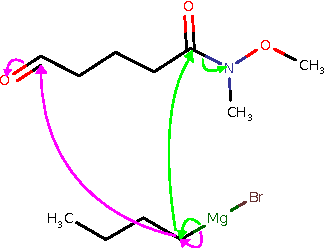
\includegraphics{imgs/textbook/reactants2}
        \caption{Predicted mechanism of our model on reactant molecules. Green arrow shows preferred mechanism, whereas pink shows the model's second preferred choice. Here, the first-choice prediction is incorrect, but chemically reasonable, as the Weinreb amide is typically used together in reactions with Magnesium species. The second-choice prediction is correct.}
        \label{fig:extra-textbook-example}
\end{figure*}

\begin{figure*}[h]
        \centering
        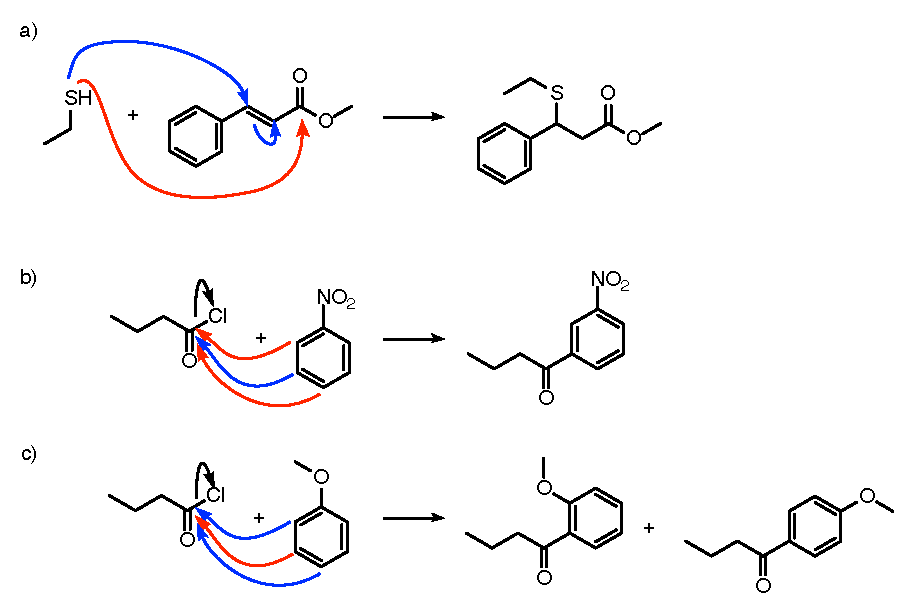
\includegraphics[width=0.7\textwidth]{imgs/textbook/additionalexamples.eps}
        \caption{Additional typical selectivity examples: Here, the expected product is shown on the right. The blue arrows indicate the top ranked paths from our model, the red arrows indicate other possibly competing but incorrect steps, which the model does not predict to be of high probability. In all cases, our model predicted the correct products. In b) and c), our model correctly recovers the regioselectivity expected in electrophilic aromatic substitutions.}
        \label{fig:extra-textbook-example2}
\end{figure*}




\begin{figure*}[h]
        \centering
        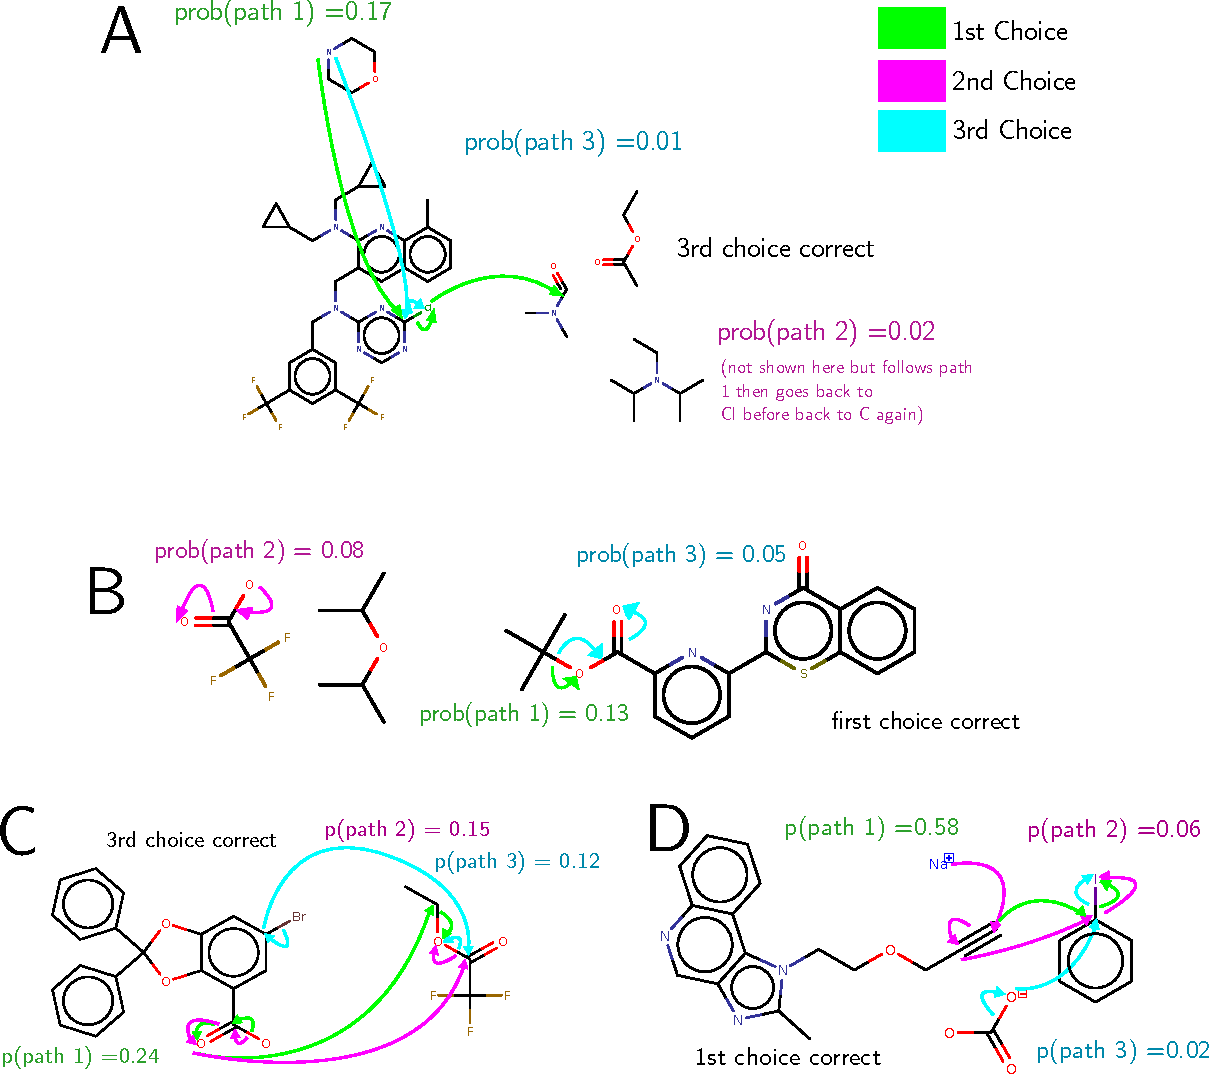
\includegraphics[width=1.0\textwidth]{imgs/appendix_examples}
        \caption{Four examples of the paths predicted by the \ourModelIR. (These reactions have been taken from the USPTO dataset and have not been seen by the model in training).}
        \label{fig:appendix_examples}
\end{figure*}



